\documentclass[letterpaper,12pt,fleqn]{article}
\usepackage{matharticle}
\usepackage{tikz}
\usepackage{pgfplots}
\pgfplotsset{compat=1.14}
\pagestyle{plain}
\begin{document}

\begin{center}
  \large
  Math-19 Section 1

  \Large
  Homework \#4

  \large
  \textbf{Due: 7/1/2019 9:00am}
\end{center}

\subsection*{Reading}

Sections 2.1--2.6

\subsection*{Problems}

\begin{enumerate}
\item Use the graph of $y=f(x)$ to answer the following questions:

  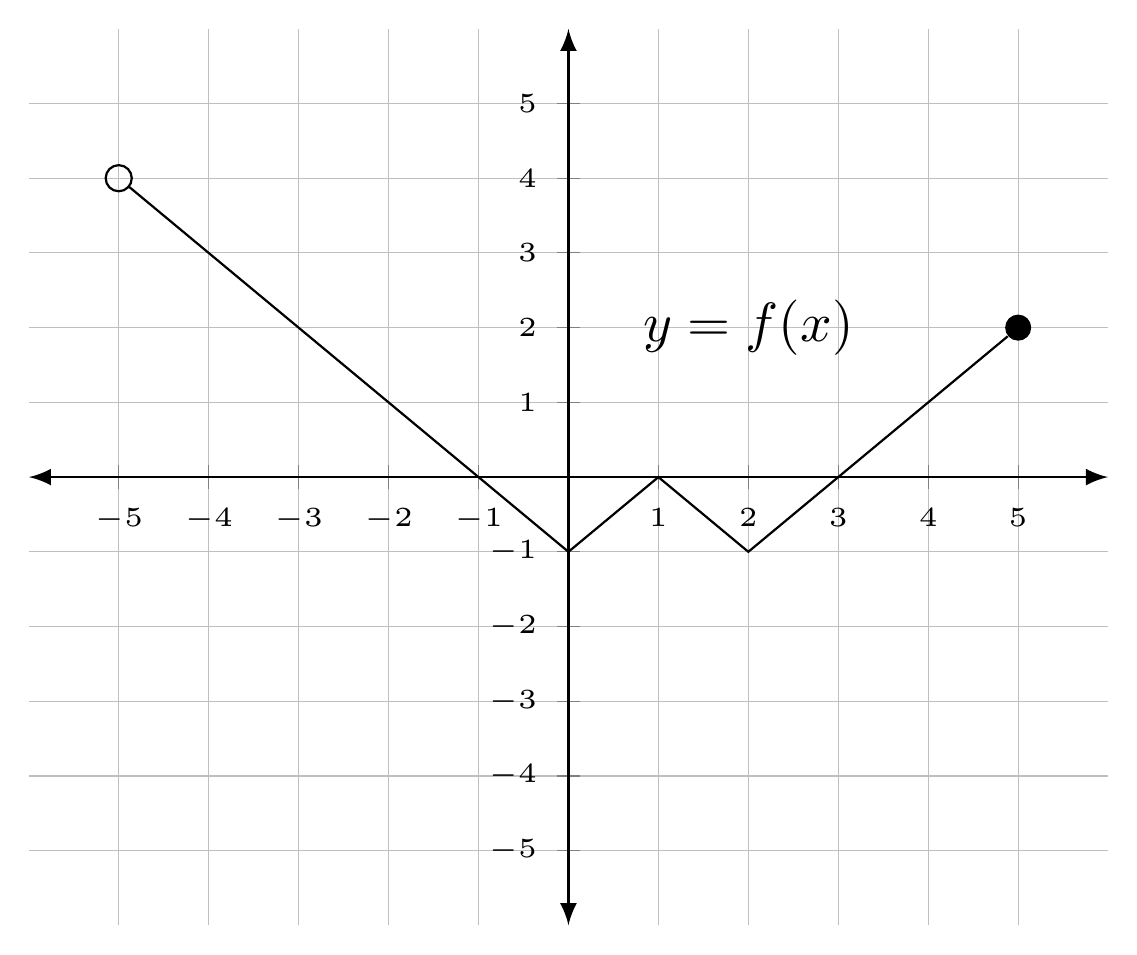
\begin{tikzpicture}[scale=2]
    \begin{axis}[
        xmin=-6,xmax=6,
        ymin=-6,ymax=6,
        grid=both,
        grid style={line width=.1pt, draw=gray!10},
        major grid style={line width=.2pt,draw=gray!50},
        axis lines=middle,
        axis line style={latex-latex},
        xtick={-5,-4,-3,-2,-1,0,1,2,3,4,5},
        ytick={-5,-4,-3,-2,-1,0,1,2,3,4,5},
        ticklabel style={font=\tiny},
      ]
      \node (a) [circle,draw,scale=0.5] at (-5,4) {};
      \node (b) [circle,fill,scale=0.5] at (5,2) {};
      \draw (a) to (0,-1) to (1,0) to (2,-1) to (b);
      \node at (2,2) {$y=f(x)$};
    \end{axis}
  \end{tikzpicture}

  \begin{enumerate}
  \item What is $f(2)$?
  \item What is the y-intercept?
  \item For what values of $x$ is $f(x)=0$?
  \item What is the domain of $f$, in interval notation?
  \item What is the range of $f$, in interval notation?
  \item On what intervals is $f$ increasing?
  \item On what intervals is $f$ decreasing?
  \item What are the local minima (if any)?
  \item What are the local maxima (if any)?
  \item What is the absolute maximum (if any)?
  \end{enumerate}

\item Consider the function: $y=-2\abs{x-2}+3$
  \begin{enumerate}
  \item List the starting standard function and the four transformation steps in the order that they should be
    applied.
  \item What are the $x$-intercepts (if any)?
  \item What are the $y$-intercepts (if any)?
  \item What are the local maxima (if any)?
  \item What are the local minima (if any)?
  \item What is the domain?
  \item What is the range?
  \item What is the axis of symmetry?
  \item Sketch the graph of the function. Be sure to label all important points.
  \end{enumerate}
\end{enumerate}

\end{document}
